\documentclass{article}
\usepackage[utf8]{inputenc}
\usepackage{amsmath, amssymb, amsthm}
\usepackage{graphicx, float}
\graphicspath{{./Imagens/}}
\usepackage{multicol}
\usepackage[brazil]{babel}
\usepackage{pgfplots}
\pgfplotsset{compat=1.18}
\usepackage[letterpaper, top = 1in, bottom = 1.0 in, left = 0.8 in, right = 0.8 in, heightrounded]{geometry}

%%%%%%%%%%%%%%%%%%%%%%%%% Caso haja dúvidas na Symbologia %%%%%%%%%%%%%%%%
% https://detexify.kirelabs.org/classify.html
%%%%%%%%%%%%%%%%%%%%%%%%% Parâmetros de construção %%%%%%%%%%%%%%%%%%%%%%%

\setlength{\parindent}{0pt}
\setlength{\parskip}{0.8em}

\title{\textbf{Repositório de Cálculo Numérico}}
\author{UFSC Joinville - EMB5016 \\ Artur Gemaque}
\date{\today}
%%%%%%%%%%%%%%%%%%%%%%%%%% COMEÇO DO DOCUMENTO %%%%%%%%%%%%%%%%%%%%%%%%%%%
\begin{document}
\maketitle

\begin{abstract}
    Este documento tem a finalidade de repositório atuando como material de reforço 
    para os alunos da disciplina de Cal. Numérico do professor Alexandre Zabot. Nesse sentido, 
    devo informar que os sequintes conteúdos são nada mais do que anotações 
    dos alunos no decorrer das aulas. Agradecimentos ao Maicon que me deu essa ideia!
\end{abstract}

\begin{multicols}{2}

\section{Aproximações de raizes}
    \subsection{Bissecção}
        O método divide repetidamente pela metade (bisseção) subintervalos de [a, b] e, em cada
        passo, localiza a metade que contém p, sendo p a raiz da equação.

        O método consiste em: 
        \begin{enumerate}
            \item Chute um valor para "a"\ e outro para "b", de maneira que $ f(x) $ seja continua no intervalo [a,b].
            \item Atribua o valor médio de "a"\ e "b"\ a uma variável chamanda de "q".
            \item Certifique-se que "q"\ não é uma raiz.
            \item Verifique o sinal de $ f(a) $ e $ f(q) $.
            \item Caso I. $ f(a) $ e $ f(q) $ contém mesmo sinal $\Longrightarrow $ A raiz está entre "q"\ e "b". 
            \item Substitua "a"\ pelo valor de "q"
            \item Retorne para o iten 2
            \item Caso II. $ f(a) $ e $ f(q) $ contém sinais opostos $\Longrightarrow $ A raiz está entre "a"\ e "q". 
            \item Substitua "b"\ pelo valor de "q"
            \item Retorne para o iten 7
        \end{enumerate}

    \subsection{Iteração de Ponto Fixo}
        Observamos que sempre podemos reescrever uma equação da forma $ f(x) = 0 $, de modo que obtamos a função equivalente $ g(x) = x^* $ 
        . Por exemplo:

        \begin{enumerate}
            \item $ e^x = x + 2 $, podemos reescrever como $ f(x) = 0 $ ou $ f(x) = e^x - x - 2 $
            \item Reescrevemos a função que representa todos os "0" da equação como x = x da sequinte forma $ g(x) = x $ e $ g(x) = e^x - 2 $ 
            \item Dada uma função $ g(x) $, a iteração do ponto fixo consiste em computar a seguinte sequência recursiva: \\ $ x^{(n+1)} = g(x^{(n)}),\  n >= 1, $
        \end{enumerate}

    \subsection{Método de Newton}
        if you have a equation named by $ f(x) = cos(x) + 1$ and want to apply the Newton's Method, follow the steps

        %\colorbox{yellow}{hello}
        
        \begin{enumerate}
            \item Find the $ f'(x) = \frac{d(f(x))}{dx} \rightarrow f'(x) = -sen(x) $
            \item Utilize the equation $ x_{n+1} = x_n - \frac{f(x_n)}{f'(x_n)} $ 
            \item Enter an approximate value for $ x_0 $, nesse caso 
            \item $ x_1 =  2 - \frac{cos(2) + 1}{-sen(2)} \rightarrow x_1 = 2,64209 $
            \item $ x_1 =  2,64209 - \frac{cos(2,64209) + 1}{-sen(2,64209)} \rightarrow x_1 = 2,89716 $
            \item $ x_1 =  2,89716 - \frac{cos(2,89716) + 1}{-sen(2,89716)} \rightarrow x_1 = 3,01999 $
            \item $ x_1 =  3,01999 - \frac{cos(3,01999) + 1}{-sen(3,01999)} \rightarrow x_1 = 3,08086 $
            \item $ x_1 =  3,08086 - \frac{cos(3,08086) + 1}{-sen(3,08086)} \rightarrow x_1 = 3,12641 $
            \item The result tends to $ \pi $
        \end{enumerate}

\section{Resolução de Matrizes}
        \subsection{Método Gaussiano, ou método de \\escalonamento}
        Este método consiste em aplicar sucessivas operações elementares num sistema linear, para o transformar num sistema de mais fácil
        
        \begin{quote}
            Algorítimo de 3 Etapas
        \end{quote}
        \begin{enumerate}
            \item Etapa 1: Gerar uma matriz aumentada apartir de um sistema de equações:
            \item Etapa 2: 
            \begin{quote}
                1° Fase Deseja-se zerar todos os elementos da primeira coluna abaixo da diagonal principal
            \end{quote}
            \begin{quote}
                Agora, devem-se zerar todos os elementos da segunda coluna abaixo da diagonal principal
            \end{quote}
            \item Etapa 3: Resolve o sistema facilitado
        \end{enumerate}
        
        \subsection{Método de Gauss-Seidel}
        Este método consiste em manipular o sistema através de determinadas operações elementares, transformando a matriz estendida do sistema em uma matriz triangular

        \begin{quote}
            Critérios que garantem a convergência das soluções
        \end{quote}
        \begin{enumerate}
            \item Critério de Sassenfeld
            \item Critério das linhas
            \item Diagonal Principal Dominante
        \end{enumerate}

        \hbox{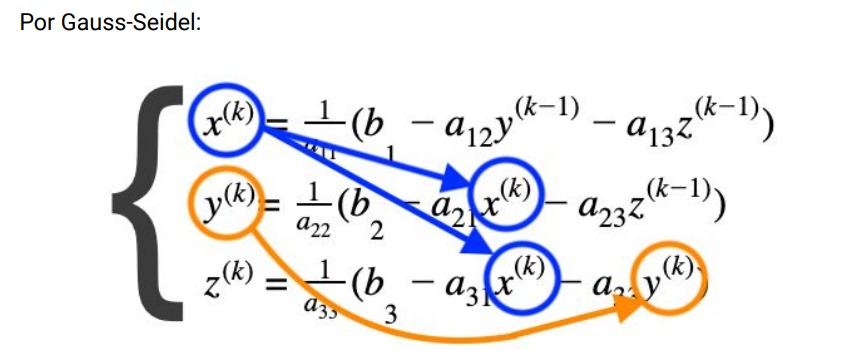
\includegraphics[width=7cm]{Gauss-Seidel.jpg}}
    
\end{multicols}
\end{document}